\documentclass{article}
\usepackage[utf8]{inputenc}
\usepackage[T1]{fontenc}
\usepackage{graphicx}
\usepackage{amsmath}
\usepackage{wrapfig}
\usepackage[top=1in, bottom=1.25in, left=1.1in, right=1.1in]{geometry}

\title{Reporte - Actividad 7: Sistema de Masas con Oscilaciones No Lineales y Forzadas}
\author{García Monge Itzel Alexia}
\date{24 de Marzo, 2018}

\begin{document}
\maketitle
\section{Introducción}
El siguiente reporte se centra en encontrar la solución de un sistema de dos resortes acoplados, contando con oscilaciones lineales, no lineales y forzamiento, siendo su solución un sistema de ecuaciones lineales de cuarto orden. Se utilizó la herramienta $Jupyter Lab$ para programar con $Python$ y lograr conseguir el valor de las ecuaciones recurriendo a métodos numéricos y graficando el resultado, seleccionando un cierto número de puntos para afinar el valor obtenido. Se comparó la solución analítica conocida y el valor aproximado de $Python$, obteniendo su error y, nuevamente, graficarlo.

\section{Síntesis}
\subsection{Introducción}
En los últimos años, la elaboración de programas que resuelven sistemas algebraicos con algoritmos numéricos de gran potencia y con la capacidad de crear gráficas fácilmente ha ayudado a crear un nuevo estándar en la búsqueda de soluciones de ecuaciones lineales, especialmente creando un enfoque en las soluciones no lineales.

Este artículo se centra en el clásico ejemplo de dos resortes con pesos atados en serie colgando a una altura específica. Asumiendo que se comportan acorde a las leyes de Hooke podemos modelar el problemas con un par de ecuaciones diferenciales lineales de segundo orden. Al diferenciar y sustituir una ecuación de la otra obtenemos que el movimiento de cada masa puede determinarse por una ecuación diferencial lineal de cuarto orden.

En una ecuación diferencial de cuarto orden podemos investigar cuándo los movimientos de las dos masas se encuentran en fase o desfase. Si variamos la constante de resorte o agregamos un factor--aunque sea mínimo--no lineal, los movimientos oscilatorios producidos actúan de una manera muy distinta a la del modelo clásico de un resorte. 

\subsection{Sistema de dos Resortes}
El modelo de dos resortes y dos masas consiste en tener un resorte con una constante de $k_1$ atado a un techo con una masa $m_1$ colgando de ella. A esta masa se le agrega un segundo resorte con constante $k_2$, colgando una masa $m_2$ bajo todo el sistema. Cuando el sistema se encuentra en equilibrio, medimos la distancia del centro de masa $m_1$ y $m_2$ hasta el equilibrio. Denominamos a las distancias $x_1$ y $x_2$, obteniendo un modelo como el que se observa en la figura siguiente.

	\begin{figure}
    \centering
    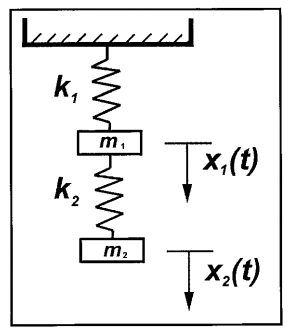
\includegraphics[height=7cm]{2spring.png}
    \caption{Dos resortes acoplados}
    \end{figure}

\subsubsection{Asumiendo la Ley de Hooke}
Si asumimos que existen pequeñas oscilaciones, las fuerzas restauradoras serían de la forma $-k_1l_1$ y $-k_2l_2$ donde $l_1$ y $l_2$ son la elongación o compresión de los resortes. 

Al estar $m_1$ conectada a los dos resortes, se tienen dos fuerzas restauradoras actuando sobre ella. Una fuerza ascendente $-k_1x_1$ ejercida por $x_1$ del primer resorte; otra fuerza ascendente $-k_2(x_2-x_1)$  ejercida de la resistencia del segundo resorte a ser comprimido o elongado por $x_2 - x_1$. Mientras que $m_2$ solo es afectada por la fuerza restauradora del segundo resorte. Al asumir que no hay fricción y usando las Leyes de Newton obtenemos un sistema de ecuaciones lineales de segundo orden de la forma

	\begin{center}
    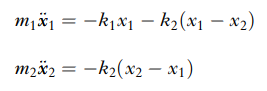
\includegraphics[height=2cm]{ec2_1.png}
    \end{center}

\subsubsection{Algunos Ejemplos con Masas Idénticas}
Para encontrar la ecuación de $x_1$ que no involucré a $x_2$, resolvemos la primera ecuación de $x_2$, despejándola para después sustituirla en la segunda ecuación diferencial. Simplificando la ecuación obtenemos 

	\begin{center}
    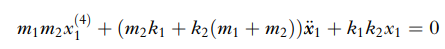
\includegraphics[height=1cm]{ec2_3.png}
    \end{center}

Repetimos el mismo procedimiento para encontrar $x_2$ y obtenemos la ecuación

	\begin{center}
    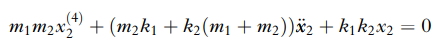
\includegraphics[height=1cm]{ec2_5.png}
    \end{center}

En ambos casos se tiene una ecuación diferencial de cuarto orden muy parecidas entre si en el movimiento de la primera masa. Es decir, los movimientos de cada masa obedecen la misma ecuación diferencial, y son solo las posiciones y velocidades iniciales las necesarias para determinar cualquier caso específico.

Si consideramos que $m_1=m_2$, asumiendo que no hay fricción ni fuerzas externas, nuestra ecuación diferencial se reduce a

	\begin{center}
    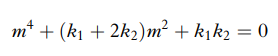
\includegraphics[height=1cm]{ec2_7.png}
    \end{center}

\textbf{\textit{Ejemplo 2.1}} 
\textit{Describe el movimiento para resortes constantes $k_1=6$ y $k_2=4$ con una condición inicial ($x_1$(0), $\dot{x}_1$(0), $x_2$(0), $\dot{x}_2$(0))=(1,0,2,0)}

Resolviendo de manera analítica, obtenemos una solución única para $x_1$ y $x_2$ que dependen de $t$:

\begin{center}
$x_1$(t)=cos$\sqrt[]{2}$t
\end{center}

\begin{center}
$x_2$(t)=2cos$\sqrt[]{2}$t
\end{center}

El movimiento que se tiene es uno sincronizado, es decir, los sistemas están en fase--se tiene el mismo periodo de movimiento pero se cuentan con diferentes amplitudes. Como el movimiento en una movimiento periódico simple, las fases de $x_1$ y $x_2$ forman elipses.

Al contar con los valores de ambas masas y constantes de resorte tenemos lo necesario para graficar el movimiento utilizando $Python$. Los demás ejemplos se graficarán de la misma forma, únicamente variando los valores de $m$, $k$ y $b$ proporcionados en el segundo segmento de código.

	\begin{center}
    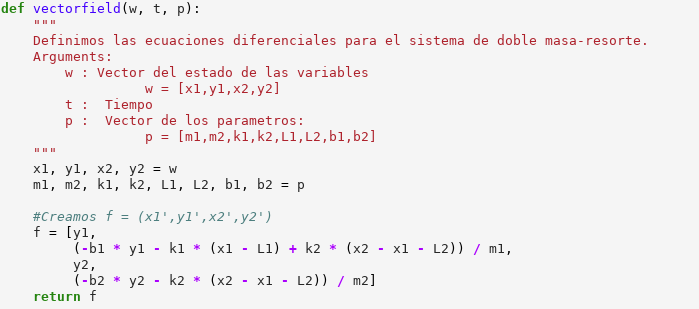
\includegraphics[height=6cm]{vecfield.png}
    \end{center}
    
    \begin{center}
    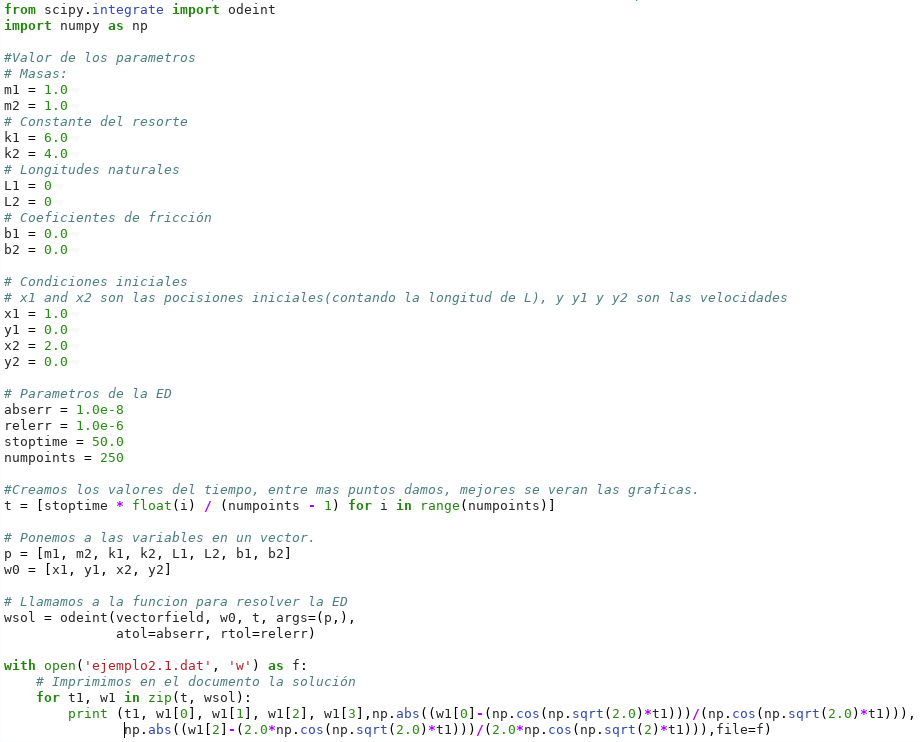
\includegraphics[height=10cm]{point21.png}
    \end{center}   
    
    \begin{center}
    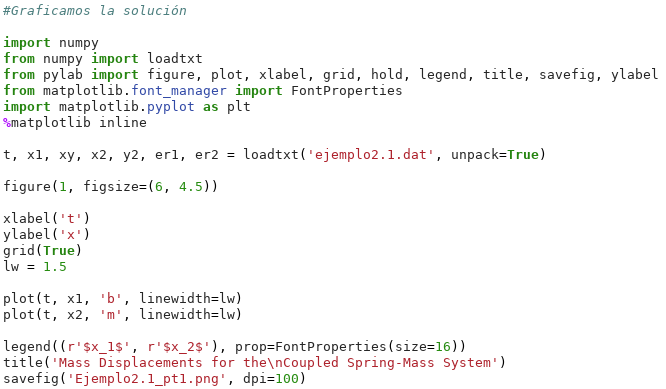
\includegraphics[height=7cm]{graf21.png}
    \end{center}
    
Obteniendo gráficas de la forma:

\begin{center}
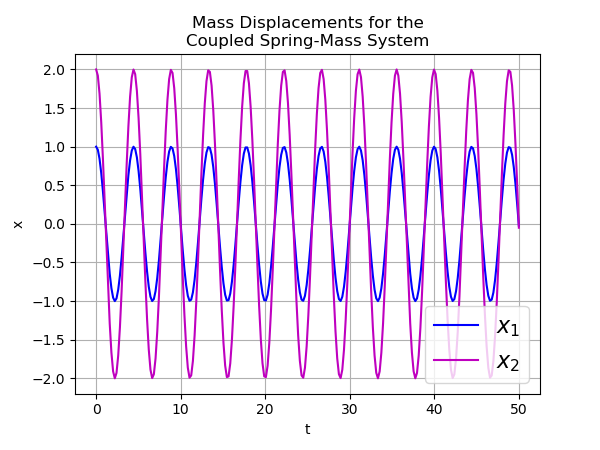
\includegraphics[height=5cm]{Ejemplo2_1_pt1.png}
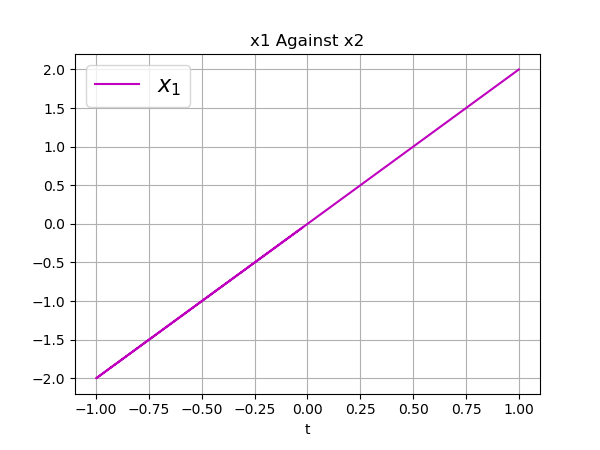
\includegraphics[height=5cm]{ejemplo2_1_p2.png}
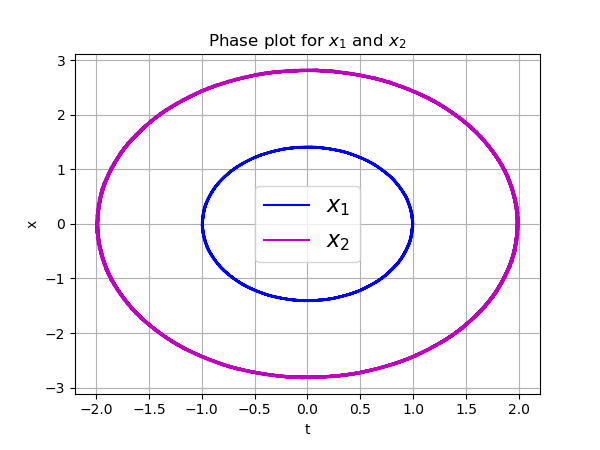
\includegraphics[height=5cm]{Ejemplo2_1_pt3.png}
\end{center}

\textbf{\textit{Ejemplo2.2}}
\textit{Describe el movimiento para la constante de los resortes $k_1$=6, $k_2$=4 con condiciones iniciales ($x_1$(0), $\dot{x}_1$(0), $x_2$(0), $\dot{x}_2$(0))=(-2,0,1,0)}

Resolvemos nuevamente de manera analítica y obtenemos una solución única para $x_1$ y $x_2$ que dependen de $t$:

\begin{center}
$x_1$(t)=-2cos2$\sqrt[]{3}$t
\end{center}

\begin{center}
$x_2$(t)=cos2$\sqrt[]{3}$t
\end{center}

Cuando $m_1$ se mueve de manera descendente, $m_2$ lo hace de manera ascendente y vice-versa. Nuevamente ambos movimientos tienen el mismo periodo, pero ahora se encuentran 180$^\circ$ fuera de fase. 

Para graficar los valores encontrados modificamos el segundo segmento de código mostrado en el ejemplo anterior

    \begin{center}
    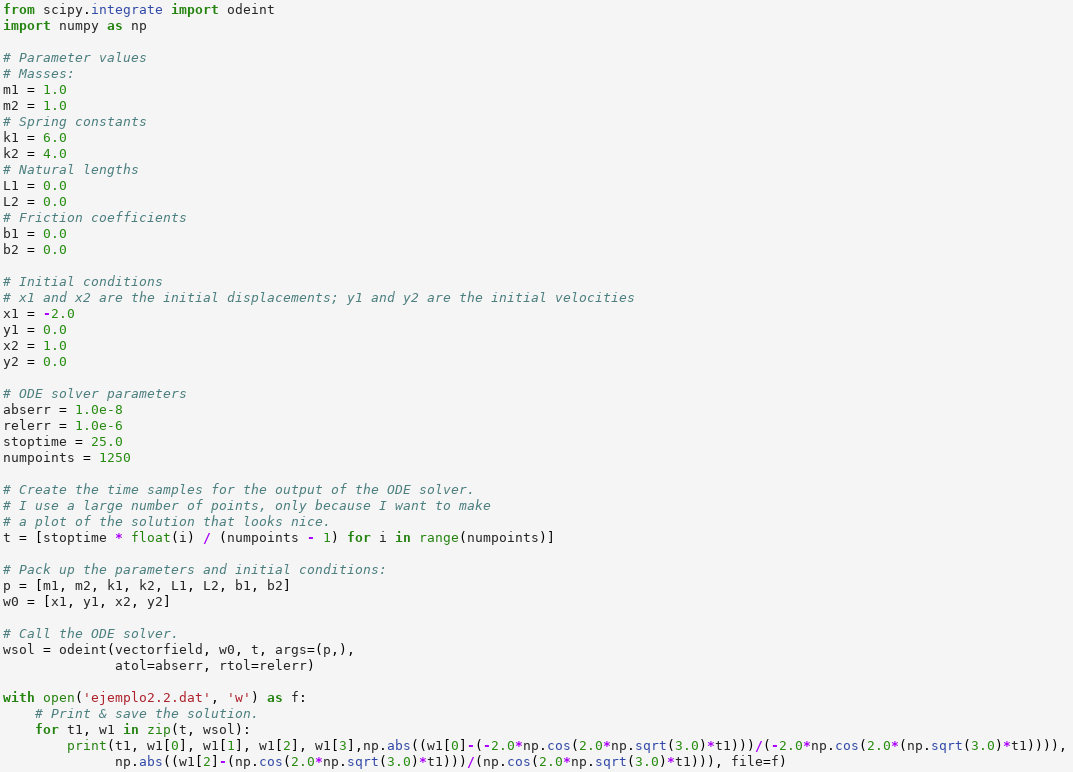
\includegraphics[height=10cm]{point22.png}
    \end{center} 

Se terminan obteniendo las siguientes gráficas:

\begin{center}
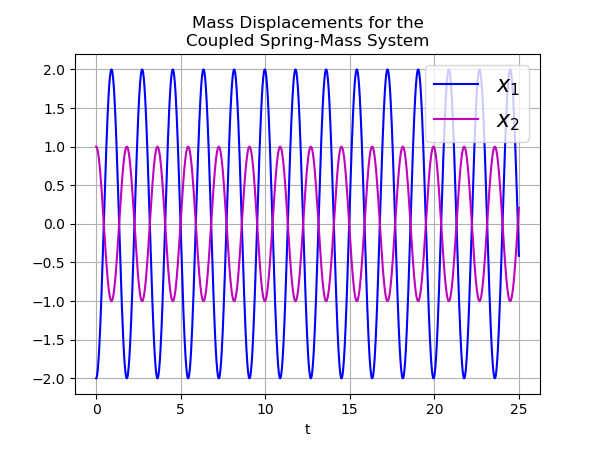
\includegraphics[height=5cm]{ejemplo2_2_p1.png}
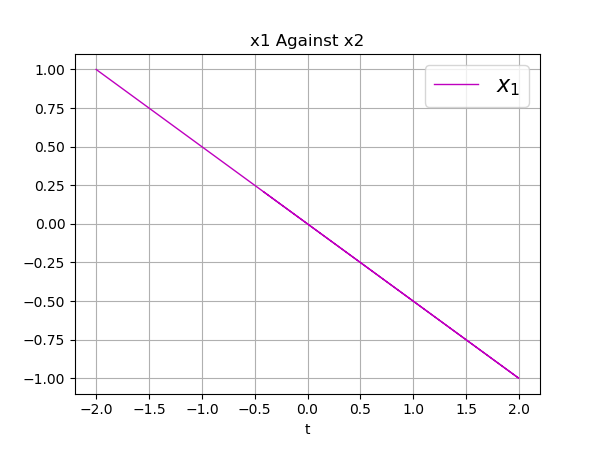
\includegraphics[height=5cm]{ejemplo2_2_p2.png}
\end{center}

\textbf{\textit{Ejemplo 2.3}}
\textit{Describe el movimiento para la constante de los resortes $k_1$=0.4, $k_2$=1.808 con condiciones iniciales ($x_1$(0), $\dot{x}_1$(0), $x_2$(0), $\dot{x}_2$(0))=(1/2,0,-1/2,7/10)}

En este ejemplo se muestra como las condiciones iniciales afectan solamente a la amplitud y fase de las soluciones. Son los valores otorgados en las constantes de resorte $k_1$ y $k_2$ las que determinan el periodo y, por ende, la frecuencia de respuesta. Sus gráficas de fase tienen casi un movimiento periódico entre ellos, y al graficar $x_1$ contra $x_2$ obtenemos una curva tipo Lissajous.

Aunque no se cuente con una respuesta analítica, aún se cuentan con las condiciones iniciales para el código.

    \begin{center}
    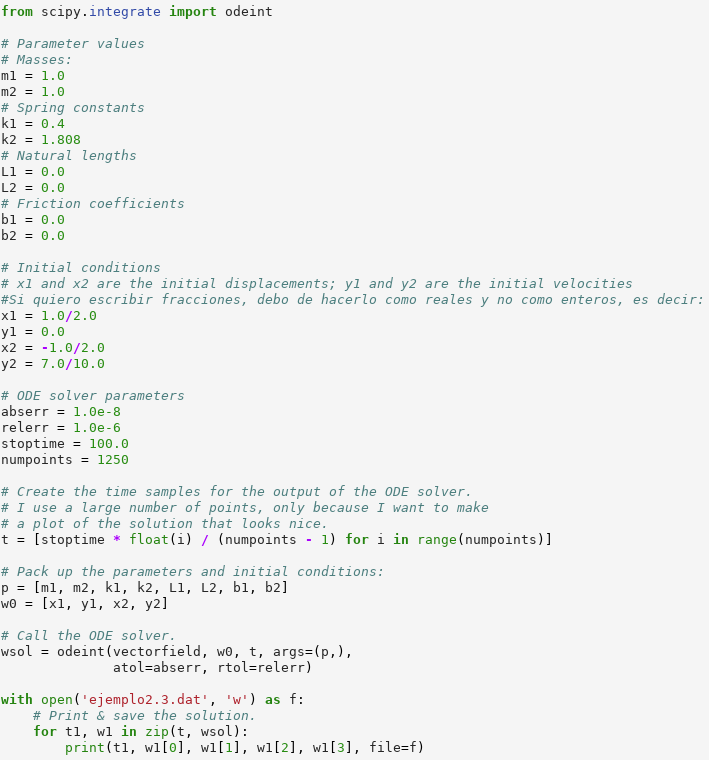
\includegraphics[height=10cm]{point23.png}
    \end{center} 

Las gráficas resultantes son

\begin{center}
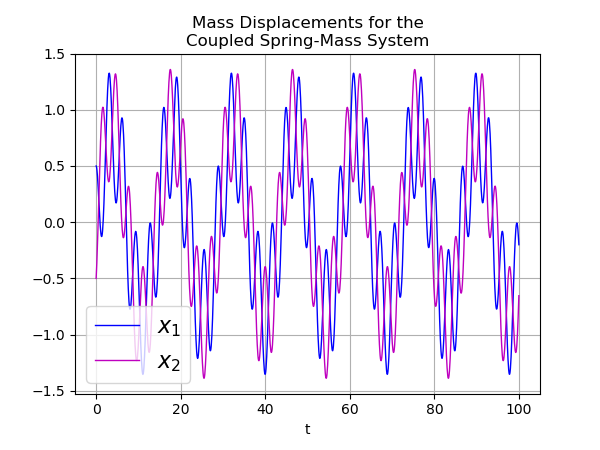
\includegraphics[height=5cm]{ejemplo2_3_p1.png}
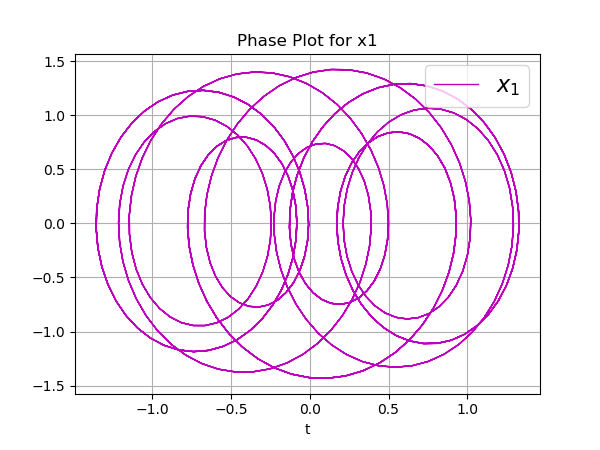
\includegraphics[height=5cm]{ejemplo2_3_pt2.png}
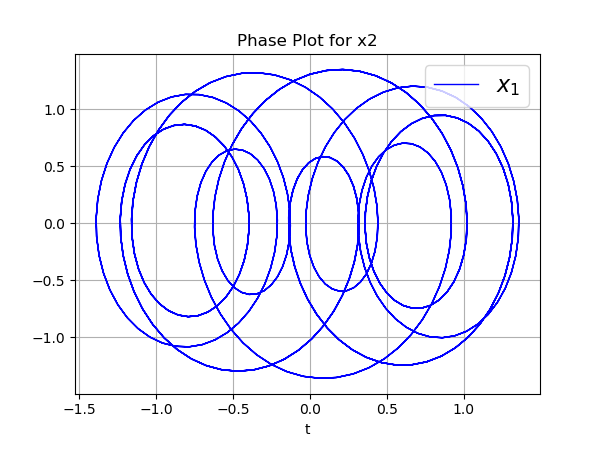
\includegraphics[height=5cm]{ejemplo2_3_pt3.png}
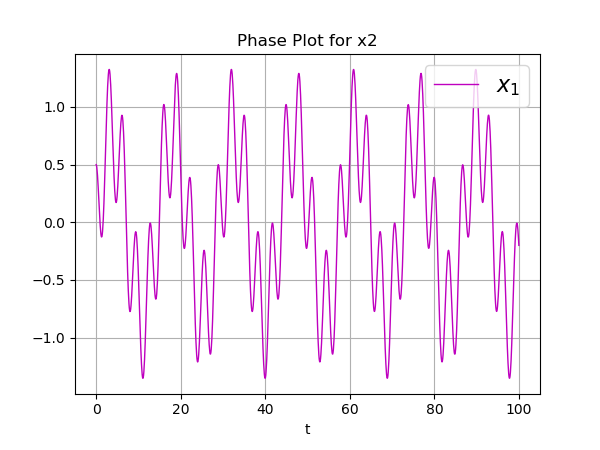
\includegraphics[height=5cm]{ejemplo2_3_pt4.png}
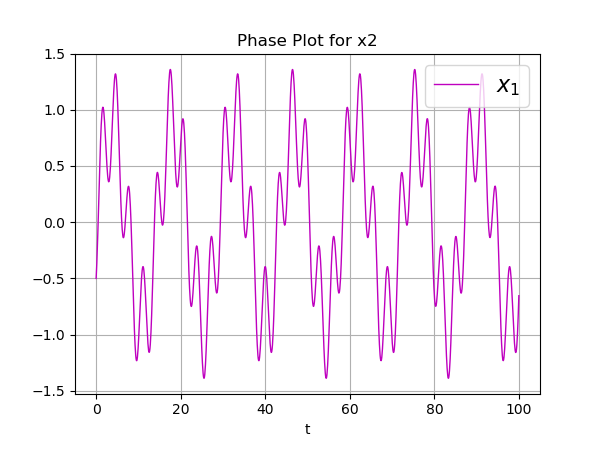
\includegraphics[height=5cm]{ejemplo2_3_pt5.png}
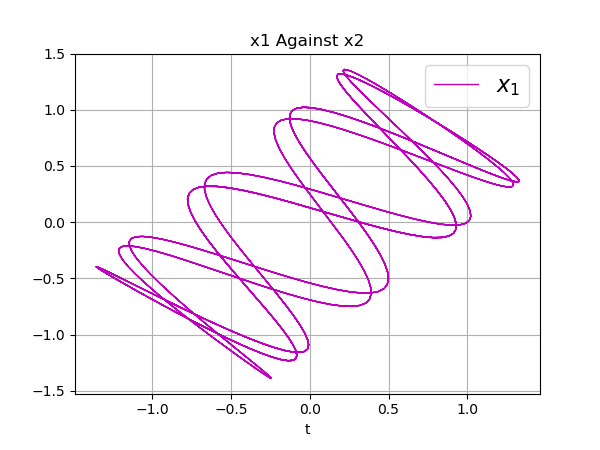
\includegraphics[height=5cm]{ejemplo2_3_pt6.png}
\end{center}

\subsubsection{Amortiguamiento}
El problema de amortiguamiento más encontrado es el de amortiguamiento viscoso, en donde el amortiguamiento es proporcional a su velocidad. El amortiguamiento en $m_1$ depende solamente en su velocidad, no en la velocidad de $m_2$ y vice-versa. 

Agregamos el amortiguamiento viscoso como $\delta$ al modelo que hemos construido  asumiendo que $\delta$$_1$ y $\delta$$_2$ son valores pequeños. Esto transforma nuestras ecuaciones iniciales en

\begin{center}
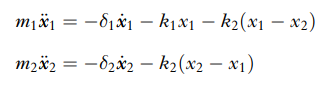
\includegraphics[height=2cm]{ec2_16.png}
\end{center}

Volvemos a realizar el procedimiento inicial, despejando $x_2$ de la primera ecuación y sustituyéndola en la segunda para conseguir una ecuación con $x_1$ que no dependa de $x_2$ y repetimos el proceso con $x_1$. El resultado que obtenemos es la misma ecuación diferencial lineal representando el movimiento de dos masas, consiguiendo movimientos de oscilaciones amortiguadas bajo simples suposiciones en los parámetros. 

\textbf{\textit{Ejemplo 2.4}}
\textit{Asume que $m_1$=$m_2$=1. Describe el movimiento para la constante de los resortes $k_1$=0.4, $k_2$=1.808, coeficientes de amortiguamiento $\delta$$_1$=0.1 y $\delta$$_2$ con condiciones iniciales ($x_1$(0), $\dot{x}_1$(0), $x_2$(0), $\dot{x}_2$(0))=(1,1/2,2,1/2)}

En el retrato de fase para $x_1$ y $x_2$ se puede observar un patrón de movimiento con amplitud decreciendo. El movimiento del amortiguamiento oscilatorio es evidente al graficar  $x_1$ y $x_2$, mientras que al graficar ambas posiciones contra el tiempo encontramos movimientos casi sincronizados, por último, $x_1$ contra $x_2$ encontramos un movimiento de oscilación amortiguada de ambas masas. 

Los cambios que sufrió el segundo segmento de código para graficar estos casos se aprecian a continuación.

\begin{center}
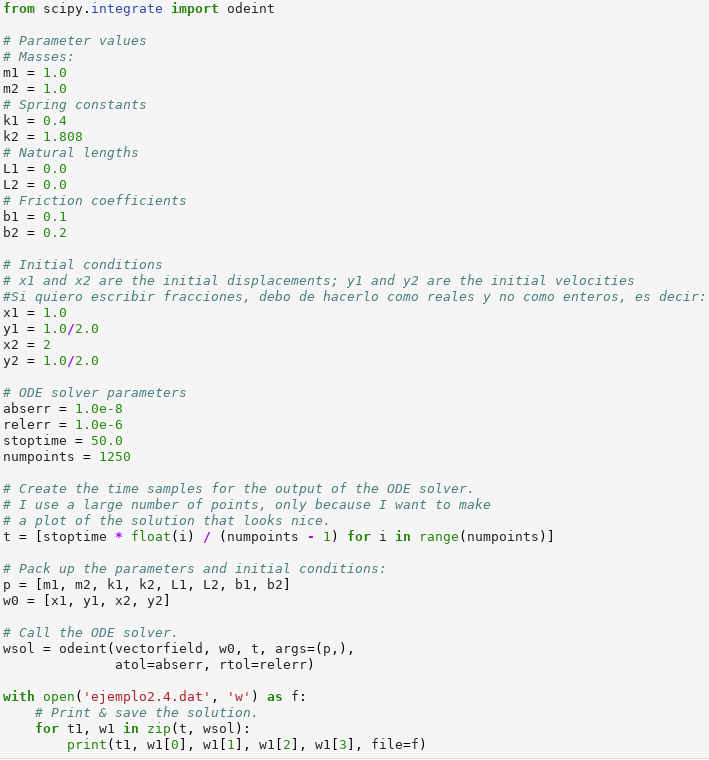
\includegraphics[height=10cm]{point24.png}
\end{center}

Las gráficas resultantes fueron:

\begin{center}
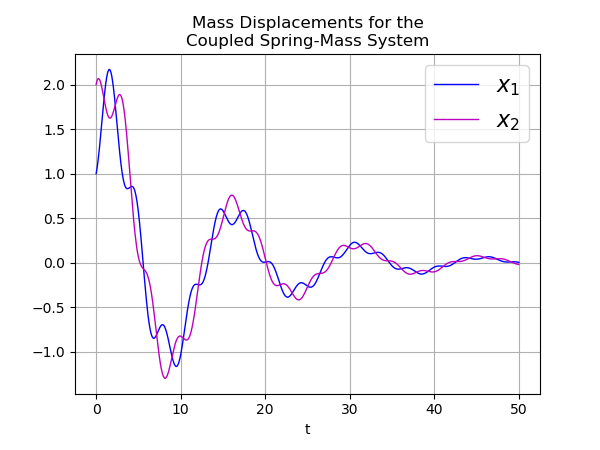
\includegraphics[height=5cm]{ejemplo2_4_pt1.png}
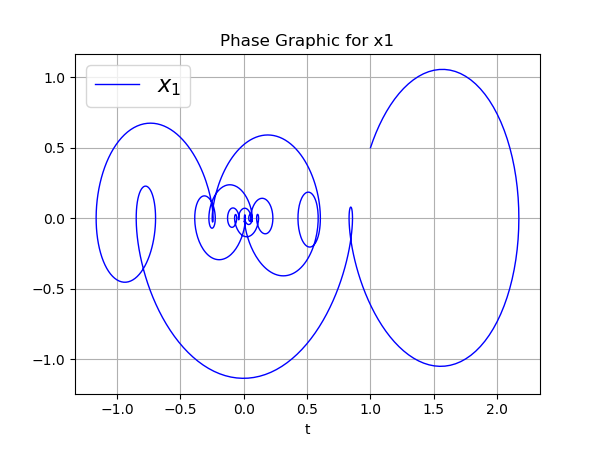
\includegraphics[height=5cm]{ejemplo2_4_pt2.png}
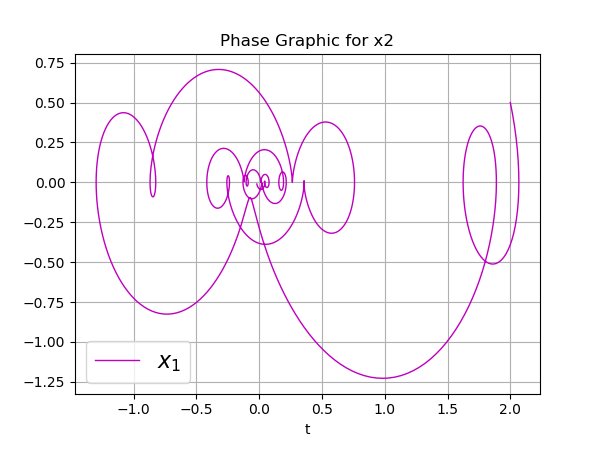
\includegraphics[height=5cm]{ejemplo2_4_pt3.png}
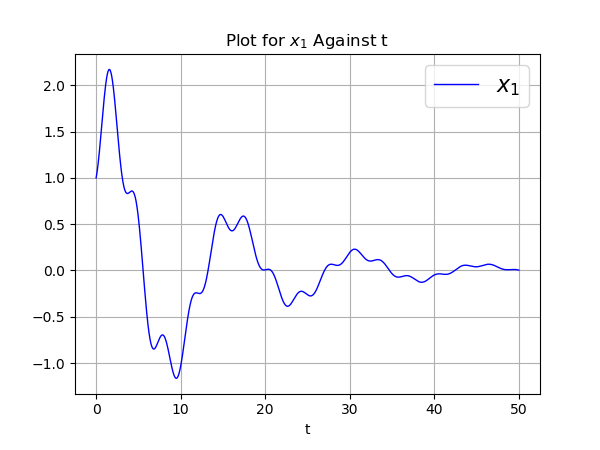
\includegraphics[height=5cm]{ejemplo2_4_pt4.png}
\end{center}

\subsection{Añadiendo No Linealidad}
Si asumimos que las fuerzas restauradoras son no lineales, estas ya no obedecen la Ley de Hooke y nuestra fuerza restauradora deja de ser $-kx$. En cambio, se obtiene una nueva fuerza restauradora, creando un nuevo modelo de ecuaciones de la forma:

\begin{center}
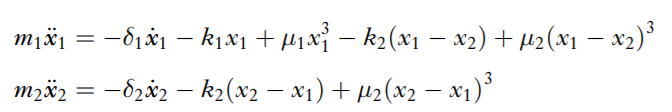
\includegraphics[height=2cm]{ec_3_1.png}
\end{center}

El rango de movimiento para los modelos no lineales se vuelve más complicado que los modelos lineales, siendo la precisión un factor importante al solucionar este tipo de ecuaciones. No hay ningún solucionador no numérico que se pueda esperar mantener preciso después de largos intervalos de tiempo.

\textbf{\textit{Ejemplo 3.1}}
\textit{Asume $m_1$=$m_2$=1. Describe el movimiento para las constantes de resorte $k_1$=0.4 y $k_2$=1.808, coeficientes de amortiguamiento $\delta$$_1$=0 y $\delta$$_2$=0, coeficientes no lineales $\mu$$_1$=-1/6 y $\mu$$_2$=-1/10, con condiciones iniciales ($x_1$(0), $\dot{x}_1$(0), $x_2$(0), $\dot{x}_2$(0))=(1,0,-1/2,0)}

Al no tener amortiguamiento, los movimientos son oscilatorios y parecen ser periódicos. Además, debido a la no linealidad, el modelo puede mostrar sensibilidad a las condiciones iniciales.

Para lograr graficar ecuaciones no lineales, no basta con modificar el segundo segmento de código como comúnmente lo hicimos en los ejemplos anteriores, pues la ecuación ya no es la misma. Tomando en consideración la no linealidad, las primeras celdas de código se vuelven de la forma siguiente.

\begin{center}
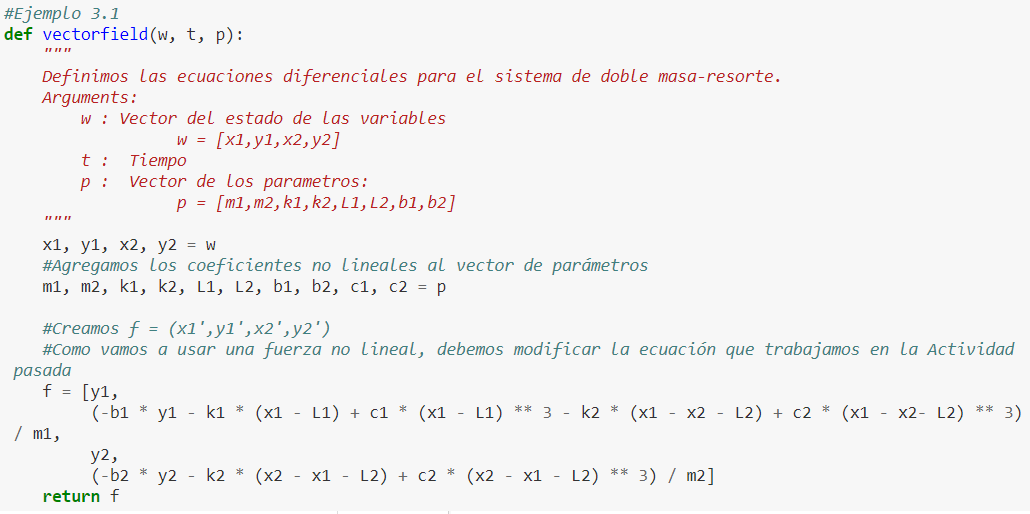
\includegraphics[height=7cm]{vecfiel2.png}
\end{center}

\begin{center}
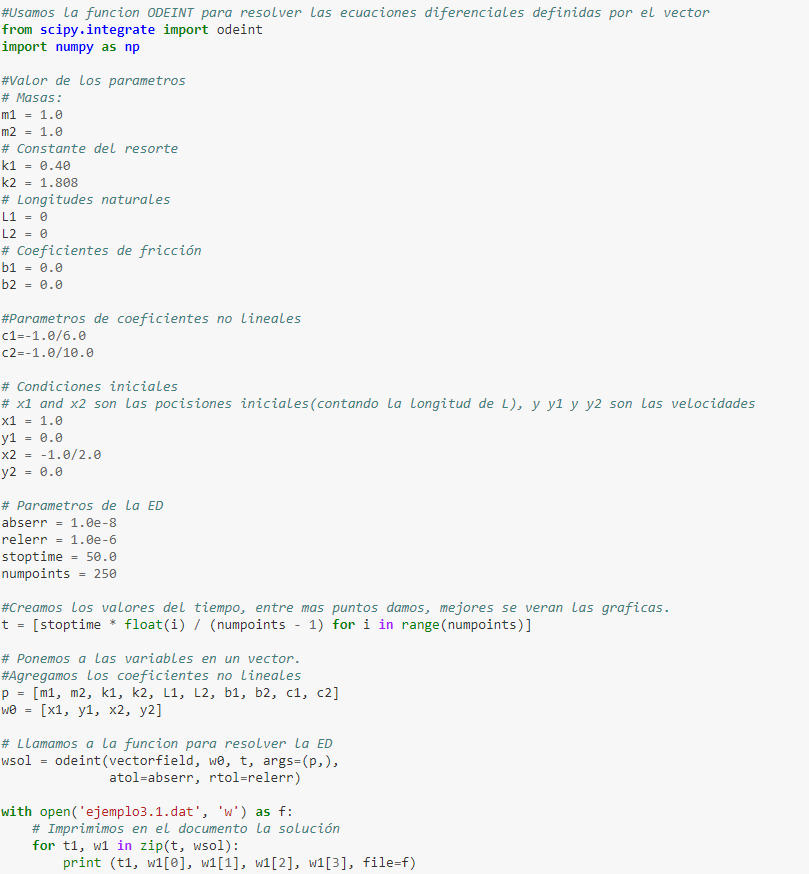
\includegraphics[height=15cm]{point31.png}
\end{center}

La tercera celda no recibe ninguna modificación, siendo la primera y la segunda necesarias al presentarse un cambio en el sistema de ecuaciones en donde se añadieron nuevos factores. Para los siguientes ejemplos nuevamente se mantienen todas las celdas iguales a excepción de la segunda. 

Las gráficas obtenidas en este ejemplo fueron:

\begin{center}
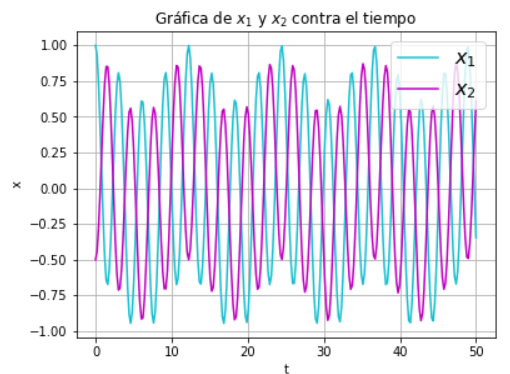
\includegraphics[height=5cm]{ejemplo3_1_pt1.png}
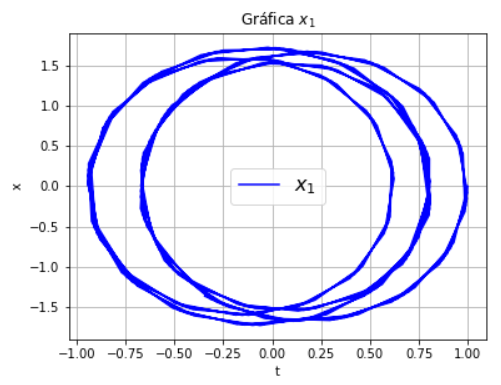
\includegraphics[height=5cm]{ejemplo3_1_pt2.png}
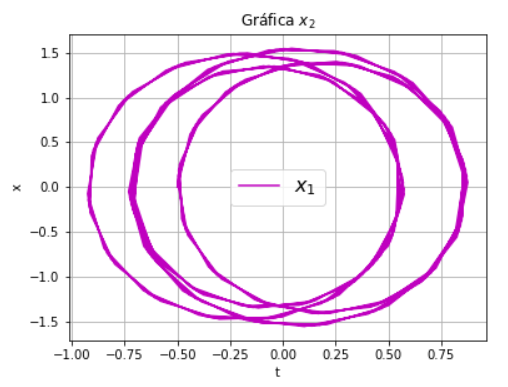
\includegraphics[height=5cm]{ejemplo3_1_pt3.png}
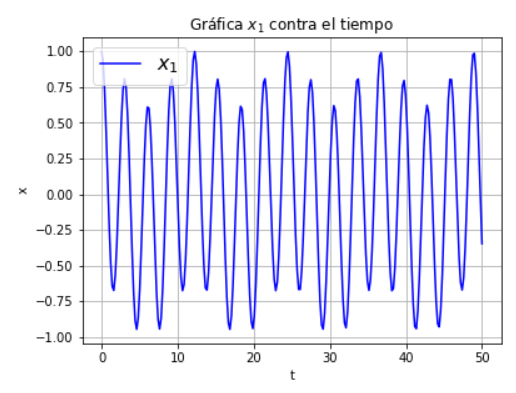
\includegraphics[height=5cm]{ejemplo3_1_pt4.png}
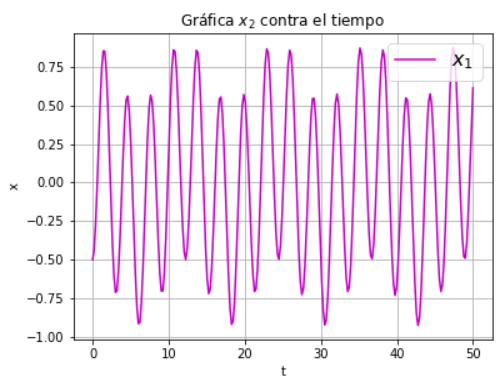
\includegraphics[height=5cm]{ejemplo3_1_pt5.png}
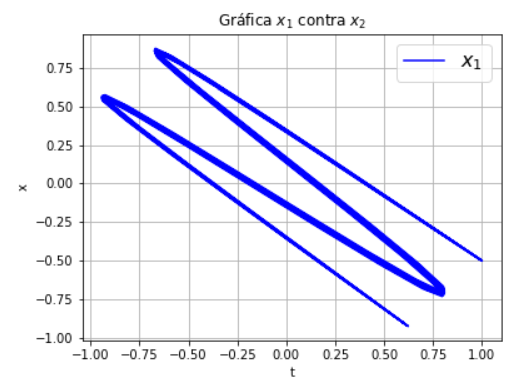
\includegraphics[height=5cm]{ejemplo3_1_pt6.png}
\end{center}

\textbf{\textit{Ejemplo 3.2}}
\textit{Asume $m_1$=$m_2$=1. Describe el movimiento para las constantes de resorte $k_1$=0.4 y $k_2$=1.808, coeficientes de amortiguamiento $\delta$$_1$=0 y $\delta$$_2$=0, coeficientes no lineales $\mu$$_1$=-1/6 y $\mu$$_2$=-1/10, con condiciones iniciales ($x_1$(0), $\dot{x}_1$(0), $x_2$(0), $\dot{x}_2$(0))=(-0.5,1/2,3.001,5.9)}

En este ejemplo no tenemos casi ningún cambio con el ejemplo anterior, solo modificamos las condiciones iniciales. Aún así, las gráficas que obtenemos como resultado son completamente distintas a las anteriores.

\begin{center}
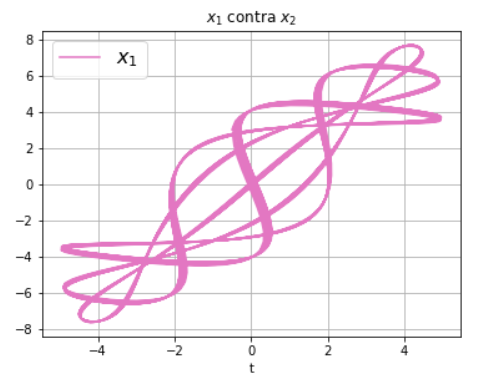
\includegraphics[height=5cm]{ejemplo3_2_pt1.png}
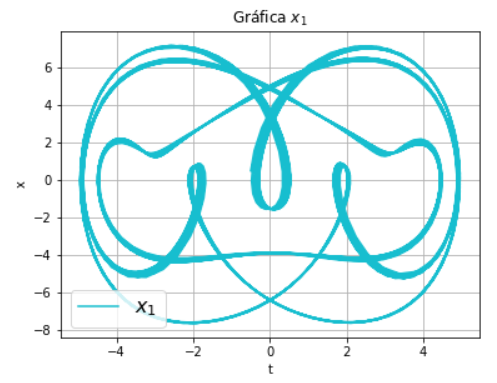
\includegraphics[height=5cm]{ejemplo3_2_pt2.png}
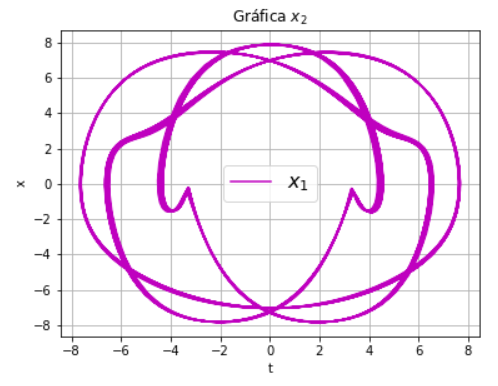
\includegraphics[height=5cm]{ejemplo3_2_pt3.png}
\end{center}

\textbf{\textit{Ejemplo 3.3}}
\textit{Asume $m_1$=$m_2$=1. Describe el movimiento para las constantes de resorte $k_1$=0.4 y $k_2$=1.808, coeficientes de amortiguamiento $\delta$$_1$=0 y $\delta$$_2$=0, coeficientes no lineales $\mu$$_1$=-1/6 y $\mu$$_2$=-1/10, con condiciones iniciales ($x_1$(0), $\dot{x}_1$(0), $x_2$(0), $\dot{x}_2$(0))=(-0.6,1/2,3.001,5.9)}

En este ejemplo, el cambio que se tiene es aún más delicado, cambiando solo amente una condición inicial del valor -0.5 a -0.6, dejando el resto del problema exactamente igual. Lo que inicialmente se piensa con este tipo de cambios sería que el cambio al sistema sería mínimo, pero al observar las gráficas observamos que no importa si a la condición inicial se le ha modificado bastante o, a primera instancia, de forma insignificante. El sistema no lineal se vuelve sumamente delicado.

\begin{center}
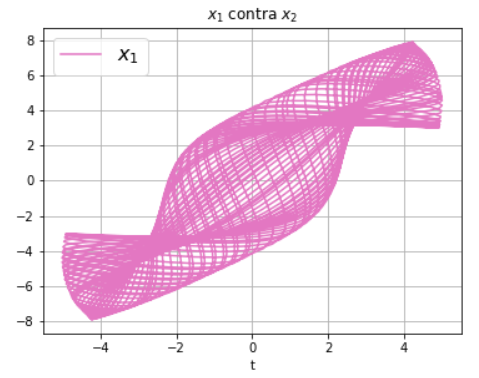
\includegraphics[height=5cm]{ejemplo3_3_pt1.png}
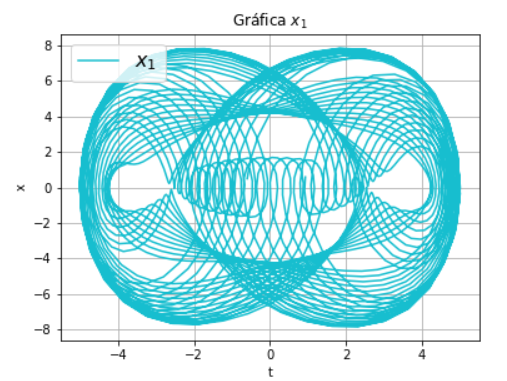
\includegraphics[height=5cm]{ejemplo3_3_pt2.png}
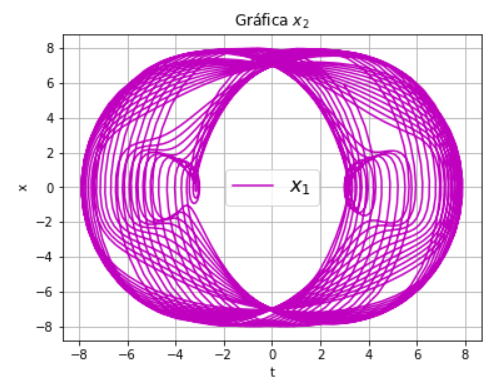
\includegraphics[height=5cm]{ejemplo3_3_pt3.png}
\end{center}

\subsection{Añadiendo Forzamiento}
Añadir una fuerza externa al modelo es algo sencillo, inclusive agregando fuerzas diferentes a cada masa. Supongamos que asumimos un forzamiento senoidal simple, nuestro modelo es modificado a

\begin{center}
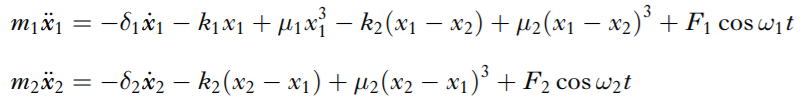
\includegraphics[height=2cm]{ec41.png}
\end{center}

El rango de movimientos para modelos de fueras no lineales es muy amplio, las condiciones en las cuales estos movimientos ocurren siendo nada fáciles de plantear. Podemos encontrarnos con resonancia no linear, soluciones armónicas, soluciones sub-armónicas y ciclos límites en el plano fase. Al cambiar la ecuación de la cual nos basamos para realizar las soluciones, volvemos a modificar las primeras dos celdas.

\begin{center}
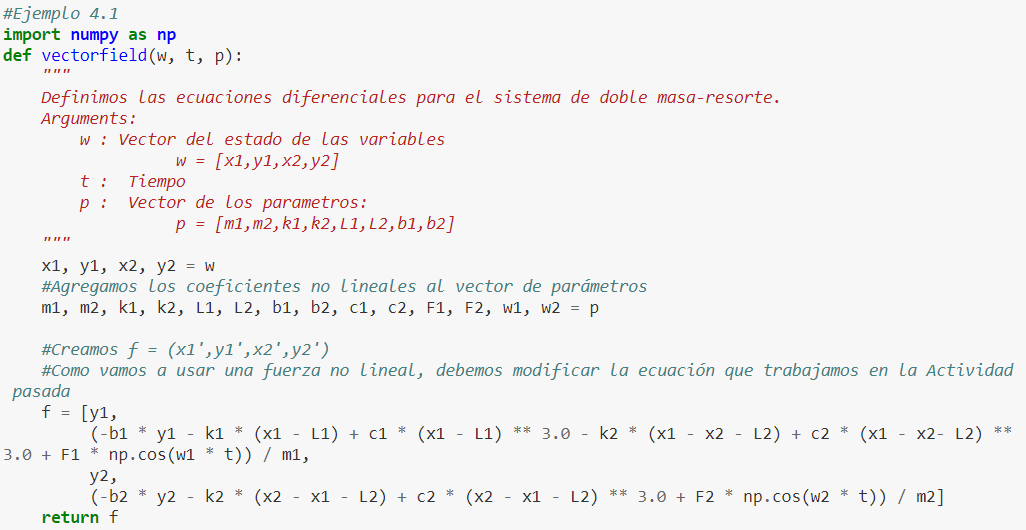
\includegraphics[height=7cm]{vecfiel3.png}
\end{center}

\begin{center}
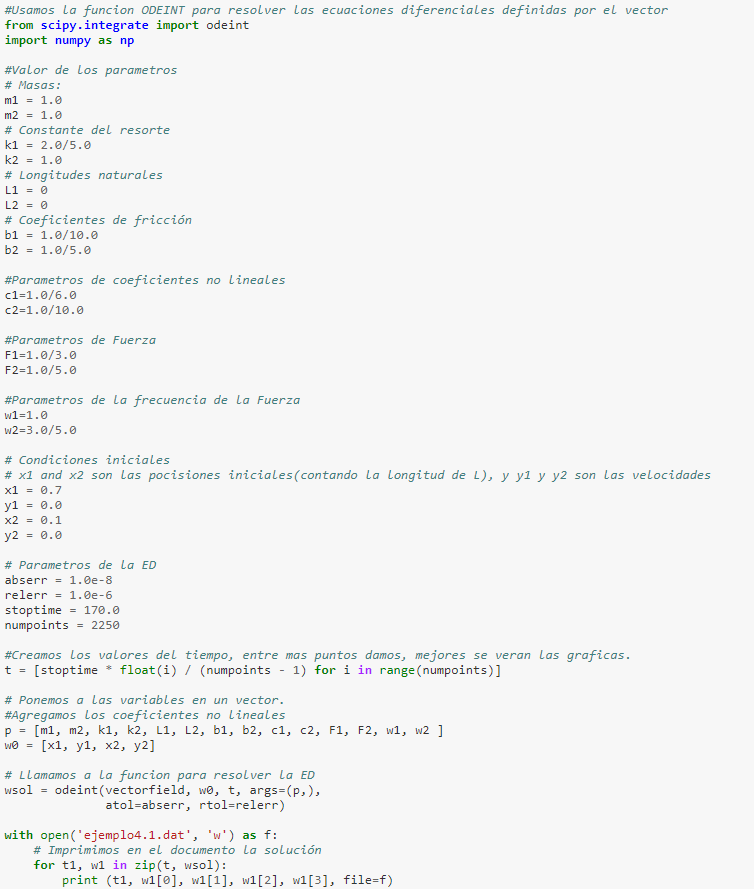
\includegraphics[height=15cm]{point41.png}
\end{center}

\textbf{\textit{Ejemplo 4.1}}
\textit{Asume $m_1$=$m_2$=1. Describe el movimiento para las constantes de resorte $k_1$=2/5 y $k_2$=1.0, coeficientes de amortiguamiento $\delta$$_1$=1/10 y $\delta$$_2$=1/5, coeficientes no lineales $\mu$$_1$=1/6 y $\mu$$_2$=1/10, amplitud de forzamiento $F_1$=1/3 y $F_2$=1/5 y frecuencias de forzamiento $\omega$$_1$=1 y $\omega$$_2$=3/5 con condiciones iniciales ($x_1$(0), $\dot{x}_1$(0), $x_2$(0), $\dot{x}_2$(0))=(0.7,0,0.1,0)}

Al contar con un coeficiente de amortiguamiento, se espera observar un comportamiento diferente para los valores pequeños de $t$ y comportamiento de estado estable para sus valores grandes. Por lo tanto, podemos esperar observar un ciclo límite en el plano fase para $x_1$ y $x_2$.

Las gráficas resultantes fueron:

\begin{center}
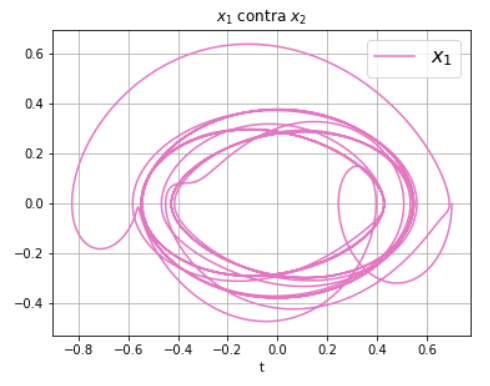
\includegraphics[height=5cm]{ejemplo4_1_pt1.png}
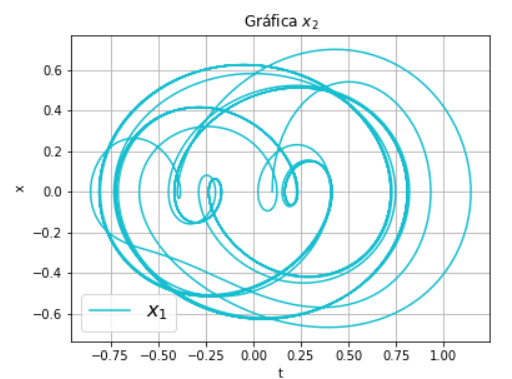
\includegraphics[height=5cm]{ejemplo4_1_pt2.png}
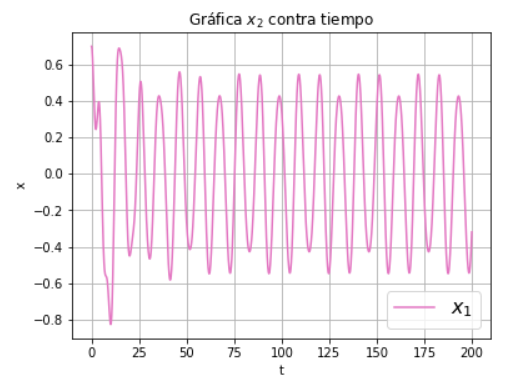
\includegraphics[height=5cm]{ejemplo4_1_pt3.png}
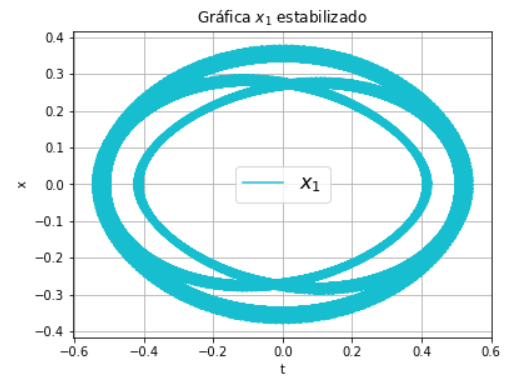
\includegraphics[height=5cm]{ejemplo4_1_pt4.png}
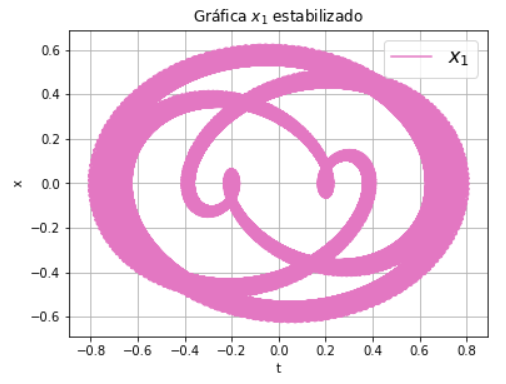
\includegraphics[height=5cm]{ejemplo4_1_pt5.png}
\end{center}

\section{Errores Relativos}
Al utilizar $Python$ para resolver sistemas de ecuaciones lineales, estamos recurriendo a métodos numéricos para encontrar el resultado. Al recurrir a métodos numéricos estamos sometiendo nuestro resultado a cierto error, pues estamos aproximando y no obteniendo el valor real como se lograría de manera analítica. Dependiendo del número de particiones que llevemos a cabo podemos acercarnos al valor real reduciendo el valor del error a uno casi insignificante.

Para los ejemplos \textit{Ejemplo 2.1} y \textit{Ejemplo 2.2} podemos encontrar el error relativo del resultado analítico restando el resultado numérico creado en $Python$ y graficarlo dependiente del tiempo. Como en  el \textit{Ejemplo 2.3} y \textit{Ejemplo 2.4} no tenemos el resultado analítico, no podemos conseguir el error relativo.

Las gráficas del error relativo en el \textit{Ejemplo 2.1} al tener 250 particiones fueron:

\begin{center}
\includegraphics[height=5cm]{error2_1_pt1.png}
\includegraphics[height=5cm]{error2_2_pt2.png}
\end{center}

Mientras que las gráficas del error relativo en el \textit{Ejemplo 2.2} al tener 1250 particiones fueron:

\begin{center}
\includegraphics[height=5cm]{error2_2_pt1.png}
\includegraphics[height=5cm]{error2_1_pt2.png}
\end{center}

En ambos casos se observan errores pequeños, obteniendo en las primeras dos gráficas un error del orden de $\times$10$^{-4}$, mientras que se obtuvo en las últimas dos un error del orden de $\times$10$^{-2}$. 

\section{Conclusión}
Al utilizar herramientas como $Jupyer Lab$, el manejo de código que realiza operaciones tan potentes como lo son las soluciones de ecuaciones diferenciales de cuarto orden se vuelven más accesibles para el público, facilitando su manejo. Podemos encontrar soluciones de ecuaciones lineales de cualquier grado al tomar como variables sus condiciones iniciales como la fricción, amortiguamiento, masa y constantes de resorte. Incluso podemos resolver ecuaciones lineales con coeficientes no lineales y forzamiento, los cuales vuelven al sistema en uno más delicado por lo cual su manejo debe ser muy cuidadoso.

Los resultados que se obtienen son siempre en base a métodos numéricos, por lo cual se debe de tener en consideración que dependiendo del número de puntos o particiones que se le designe al código se estará más cerca al valor real y, por lo tanto, se tendrá un error pequeño.  

\section{Bibliografía}
\begin{itemize}
\item Temple H. Fay, Sarah Duncan Graham (2003) Coupled Spring Equations. Int. J. Educ. Math. Sci. Tech.. Vol. 34, No. 1, pp. 65-79.

\item SciPy Cookbook. Retrieved March 18, 2018.

$http://scipy-cookbook.readthedocs.io/items/CoupledSpringMassSystem.html$
\end{itemize}


\section{Apéndice}
\begin{enumerate}
\item \textbf{¿Qué más te llama la atención de la actividad completa? ¿Que se te hizo menos interesante?} Lo fácil que es programar un sistema que me parece algo complicado plantear, en especial las partes que no son lineales. En general siento que todo era algo importante que debía prestarse atención, no hubo algo que me pareciera poco interesante.

\item \textbf{¿De un sistema de masas acopladas como se trabaja en esta actividad, hubieras pensado que abre toda una nueva área de fenómenos no lineales?} No, pues como había mencionado en la práctica anterior, solo vimos brevemente la solución de resortes acoplados en nuestro curso de Mecánica II, por lo cual no se mencionaron fenómenos de este tipo.

\item \textbf{¿Qué propondrías para mejorar esta actividad? ¿Te ha parecido interesante este reto?} Un poco de explicación en el comportamiento que tenemos de las gráficas, pues en el documento no se explica bien qué ocurre con algunas, o porque se mueve de esa forma.

\item \textbf{¿Quisieras estudiar más este tipo de fenómenos no lineales?} Me gustaría, pero primero quisiera tener un poco más de apoyo en clase para entender su programación.

\end{enumerate}
\end{document}
